\section{Summary}

  \subsection{Project Direction}
  
  The project at this point has succeeded in delivering an MVP to the product owners. However, development is not finished and is still ongoing.
  
  Current projections estimate that the project should complete its backlog within two/three more sprints, at which point a fully implemented version of the product as set out by the project's aims and objectives will be completed. This projection can be extrapolated from the cumulative flow chart shown in \autoref{fig:flow} which shows the progression of tickets under the three categories; \textit{To Do}, \textit{In Progress} and \textit{Done}.
  
  \begin{figure}[H]
    \setlength{\belowcaptionskip}{15pt plus 3pt minus 2pt}
    \caption{Cumulative Flow Chart}
    \centering
    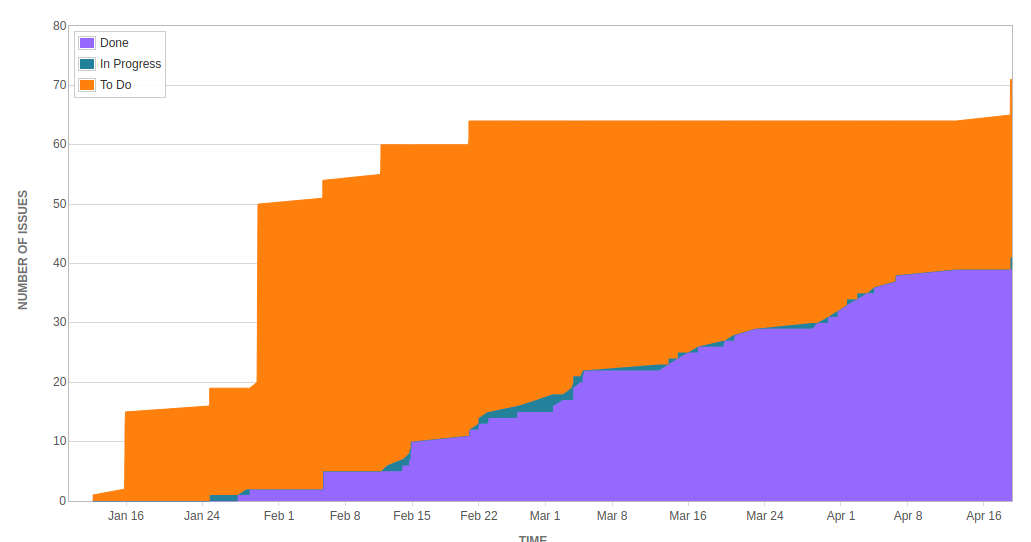
\includegraphics[width=\textwidth,keepaspectratio]{cumulative-flow}
    \label{fig:flow}
  \end{figure}
  
  This chart shows not only completion of work but also the discovery of new tasks and issues during the development  process, leading to an increase in the workload in the \textit{To Do} category. Of particular note in this chart is the significant increase in the workload that occurred in early February. This is reflective of the discussion and actions after an early retrospective with the product owners to separate the concerns of the backend API from the fronted UI. This resulted in intensive backlog refinement which included the creation of some new tickets.
  
  \subsubsection{Future Development}
  This project has been designed with future expansion of product features in mind. Indeed a noted aspect of this project is that it can currently test no relational data, but can be easily expanded to test relational data. This is facilitated by the modularity of the management servers tasks (created as Jenkins jobs) which can be interchanged as new tasks are added. For example:
  
  \begin{itemize}
    \item The task for restoring and reading data could be swapped with one which restores MySQL data instead of JSON.
    \item The decryption task (which use asymmetric cryptography) could be swapped with one which uses symmetric cryptography. 
  \end{itemize}
  Neither of these operations would affect other tasks and would be invisible to the end user.  The user could simply enter the correct setting at the dashboard and the necessary tasks would be \textit{chained} together using Jenkins Pipelines. 

	\subsection{Review}
  
  \subsubsection{Core Goals}
	This project delivered on its core goals set out by the stakeholders. In relation to its initial aims and objectives, the project has delivered the following aspects:
  
  \begin{itemize}
    \item \hyperref[ao1]{AO1:} An automated system for running a scheduling test restorations has been implemented:
    \item \hyperref[ao2]{AO2:} A notification system has been implemented to notify users of failed backups;
    \item \hyperref[ao3]{AO3:} The creation and destruction of the necessary infrastructure has been automated in order to reduce uptime and therefore also costs;
    \item \hyperref[ao4]{AO4:} Credentials have been stored and utilised in a secure manner and sensitive backup data has not been exposed;
  \end{itemize}
  
  The delivered product implemented three main components:
  \begin{itemize}
    \item A management server for the configuration and orchestration of the backup restores, implemented as a Jenkins server;
    \item A comprehensive ExpressJS API for interacting with the management server, abstracting the full configuration of Jenkins away from the user.
    \item A comprehensive frontend UI for users to use the API.
  \end{itemize}
  
  \subsubsection{Stretch Goals}
  The following stretch goals have been defined and remain on the product backlog for further development:
  
  \begin{itemize}
    \item \textbf{CLI:} Create a CLI for more advanced users who are more comfortable or proficient in command lines to use the system without visiting the user dashboard.
    \item \textbf{User Authentication: } Implement a more flexible user system which allows the addition of more users.
  \end{itemize}
  

	\subsection{Learning Outcomes}
  This project has produced a number of learning outcomes.
  
  \subsubsection{Technical Learning Outcomes}
  The following technical skills were gained or developed over the course of this project:
  
  \begin{itemize}
    \item Realised the benefits of the separation of frontend and backend through the development of a backend API and a frontend UI, emphasized through the product owners recommendation to complete one before the other as oppose to concurrently;
    \item Gained valuable insight into the containerisation of applications through researching the option of deploying multiple services to one or more containers;
    \item Learned about the CI/CD process through the implementation of a Jenkins CI/CD pipelines to build and deploy Docker images, a common software development practice in the industry when developing as part of a large team;
    \item Gained experience in developing a MEAN-stack application using ExpressJS, NodeJS and ReactJS having previously had little experience developing \textit{'full-stack'} applications;
    \item Reinforced the importance of API documentation and testing though the use of SwaggerUI;
  \end{itemize}
  
  \subsubsection{Non-Technical Learning Outcomes}
  There were also a number of  non-technical skills gained or developed over the course of this project.
  
  \begin{itemize}
    \item Learned about the benefits of project planning using Jira to define entire project workload early in the development stage.
    \item Experience was gained when dealing with a product owner. This included not only listening to their requirements and recommendation but also making decisions during development and updating the product owners accordingly.
    \item Learned how to correctly track workload and its progress with Jira. The benefits of this were emphasised later in development when enough work had been completed to compile graphs which highlighted problem areas. This helped keep the project focused on it's goal and on schedule.
    \item Communication skills improved over the course of the project as a result of regular meetings with the scrum master and product owners.
  \end{itemize}
	
  \subsection{Personal Reflection}
  As the learning outcomes above show, I feel I have gained or improved many skills while working on this project. Many of the skills I believe will be very beneficial to me in my future career. I found great satisfaction in completing and delivering the MVP as this is the largest and most comprehensive project I have undertaken.
  
  Personally I feel one of the most important learning outcomes of this project was the benefit of project planning. After the initial meeting with the product owners, at which point the main details of the project were outlined, there was a quite time-consuming and tedious job of splitting the entire project into small tasks. These tasks were then added to Jira as tickets. The granularity at which this had to be done was something I had never completed before. In previous projects I would set out \textit{To Do} lists at a much higher level, with only a few items on the list. 
  
  However, the amount of time and effort put into creating these tickets and organising them into \textit{Epics} and \textit{Issues} proved to be hugely beneficial later on in the development phase. Having the tickets created that clearly defined all the steps required to implement each user story meant I never lost focus of what I was doing. Also on completion of any given task, there was no confusion or decisions needed as to what to do next. This was always easily determined due to clearly defined tickets and a well refined backlog.
  
  I also found the prototyping stage to be of huge benefit. Initially I was unsure as to whether the project would be technically feasible. In the past I would have determined this only though beginning development and hoping to overcome issues as they arose. However, the product owners' recommendation and help in identifying the key areas of uncertainty and defining \textit{proof of concepts} accordingly was a valuable lesson. This is a lesson I will certainly remember for future projects i.e. identify problem areas before development begins and investigate their feasibility with a \textit{proof on concept} prototype.
  
  Overall I found the project to be greatly beneficial to my growth as a developer. Accordingly, I would deem the project to be a personal success with many valuable lessons learned and experiences gained. 
  
  
  